\newcommand{\h}{\unit{h}}

\section{Bilan technique}
\subsection{Justification du choix des technologies}
Le langage C++ était premièrement connu de tous les membres de l'hexanôme, de part son enseignement en 3IF, effectué plus en profondeur que celui dispensé en Java.
De plus, les connaissances acquises en dehors du cadre universitaire en C++, par plusieurs personnes ont été bénéfiques tout au long du projet, en particulier une connaissance du framework utilisé, Qt. Il s'est en effet avéré un composant essentiel lors du développement, simplifiant grandement les opérations d'affichage sur un canevas. Si le langage Java avait été choisi, nous aurions du adapter nos méthodes de programmation, ce qui aurait été positif, d'un point de vue pédagogique, mais non efficace du point de vue réalisation.

\subsection{Avantages et limites de la solution réalisée}
De part l'architecture utilisée lors de l'implémentation, une grande partie du code sera réutilisable lors d'une éventuelle utilisation hors cadre de simulation. Par exemple, la classe \kw{Chariot} pourra être remplacée par une classe se chargeant d'accéder à des capteurs physiques, et les stratégies de pilotage resteront identiques.

De plus il est d'ors et déjà, moyennant une légère modification des fichiers de configurations, d'utiliser des aiguillages possédant un nombre de sorties arbitraire.

Au niveau interface graphique, il est facile réorganiser et de modifier les contrôles, indépendamment de la base de code.
On remarquera également que le taux de rafraîchissement graphique est séparé du calcul au niveau modèle. Il est donc possible d'accélérer et de ralentir la simulation indépendamment de l'affichage, pouvant donc avoir une simulation très lente parfaitement fluide.

Qt nous apporte énormément d'avantages, mais aussi une limite : la dépendance. En effet, l'utilisation de ce framework est très intrusive ; aussi le code ne sera pas portable sur une autre technologie. C'est un choix que nous avons fait, en grande partie parce que nous savions que ce portage ne serait jamais effectué.

\section{Bilan organisationnel}
\subsection{Planning réel}
\newpage
\begin{figure}[H]
	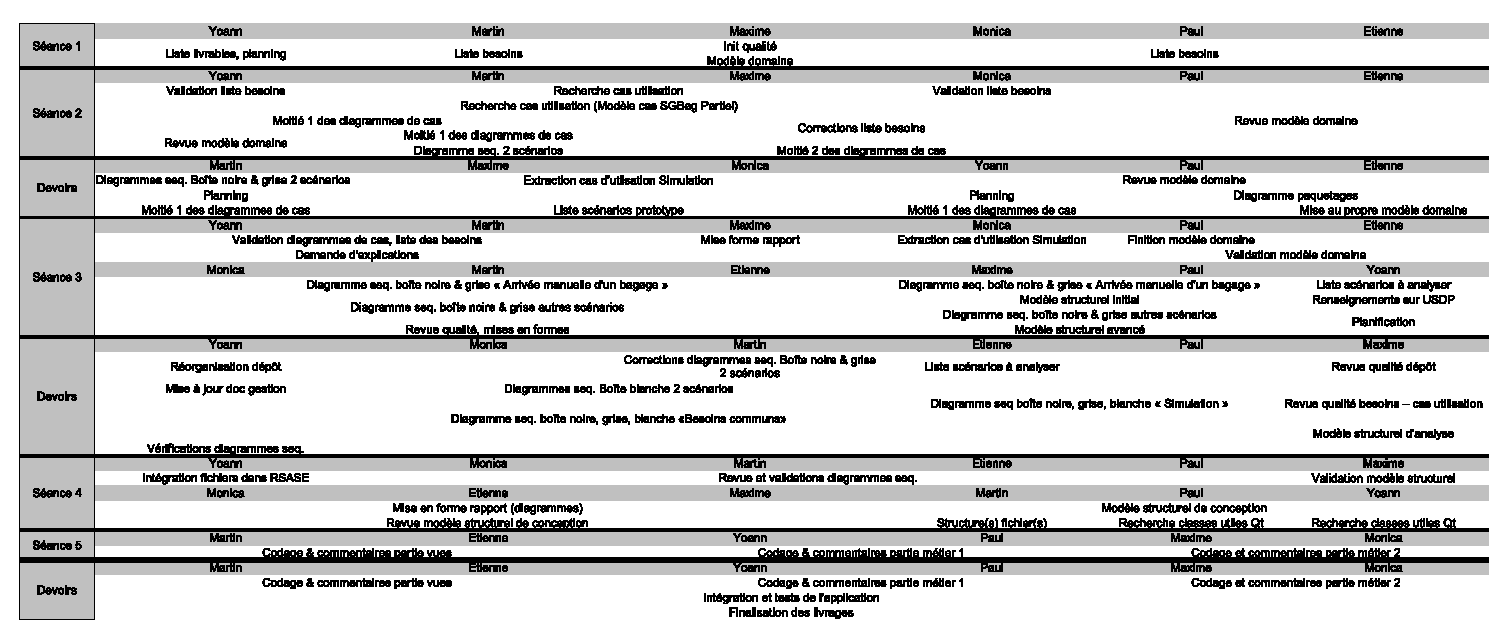
\includegraphics[width=\textwidth,angle=90]{planning2.pdf}
\end{figure}

\subsection{Temps passé sur le projet} 
\begin{tabular}{|c|c|c|c|c|c|c|}
\hline
& Martin & Maxime & Monica & Paul & Étienne & Yoann \\
\hline
Temps passé hors séance & 55 - 60\h & 35\h & 50 - 60\h & 55 - 60\h & 50 - 60\h & 60 - 70\h \\
Temps passé en séance & 15 - 16\h & 15 - 16\h & 15 - 16\h & 15 - 16\h & ?\h & 15 - 16\h \\
\hline
\end{tabular}

\subsection{Conclusions}
\subsubsection{Réflexions sur la méthode USDP}
La méthode nous a tout d'abord paru très lourde et peu accessible. En effet, il est nécessaire de bien en connaître le fonctionnement avant de la mettre en \oe uvre, voir même de l'avoir déjà expérimenté, d'un autre point de vue de celui d'un chef de projet.

Par la suite, nous avons pu constater l'intérêt de chacun des livrables, en procédant par raffinement successif, permettant de générer le code.

Cependant, l'utilisation d'outils de génération de code s'est révélée, sur ce projet, et avec les technologies choisies (Code non conforme au standard C++, puisqu'utilisant Qt), plus pénalisant que l'écriture des squelettes de code à la main. En particulier, nous ne pouvions procéder de manière itérative, ne pouvant pas effectuer de génération de diagrammes à partir du code de manière réellement efficace (c'est à dire sans modification manuelle a posteriori).

D'autre part, la méthode USDP n'est visiblement pas adaptée au dimensionnement humain, ni à la taille de ce projet. L'ensemble des phases de la méthode aurait été beaucoup plus vite réalisé si le besoin parallélisation avait été moins important (par exemple avec un nombre plus réduit de collaborateurs). Sur un projet de cette taille, l'utilisation de méthodes de type agile aurait vraisemblablement été plus adapté.

\section{Bilan personnel}
Dans l'ensemble, les membres de l'hexanôme sont d'avis que ce projet leur a apporté une connaissance plus poussée du framework Qt, et leur a donné une première expérience du travail en équipe. Ainsi, nous avons tous pu réaliser les difficultés qu'entraîne le travail en groupe et avons pu repousser nos limites durant quelques semaines relativement intenses.

Le chef de projet a quant à lui pu constater qu'il avait un goût prononcé pour le fait de ne pas être chef de projet, et ce projet lui a donc confirmé qu'une carrière d'architecte logiciel correspondrait très bien à ses compétences.

